\chapter{Implementation of a Key Management Entity}
\label{ch:implementation}%

The previous chapter introduced the Key Management Entity (KME). Then, we described its interaction with Secure Application Entities (SAEs) and Quantum Channels (QCs). Next, we focused on the internal functioning of the KME, finally giving a complete overview of the key management process.

This chapter will focus on our implementation of a Key Management Entity.

The KME is implemented using Python \cite{python}, one of the most popular high-level programming languages nowadays. In particular, this implementation works only with a version of Python at least equal to 3.10, the most recent version at the time of writing.

In the following sections, we will introduce Poetry, the dependency management system of this project. Then, we will describe the software dependencies required to make this KME implementation work. After that, we will explain how to start one KME or a couple of cooperating KMEs. Next, we will describe the different modes of operation of the KME: development, testing, and production. In the end, we will focus on how the project has been tested.

\section{Software dependencies}

Within a software project, recurring problems are encountered. The solutions to these problems are pieces of software that developers reuse in multiple projects, at the cost of not having complete control over their development. They are called "dependencies".

The dependency management of this project is entrusted to Poetry. Poetry reads the project dependencies from a file called \textit{pyproject.toml}, and it allows to install all of them with a single command:

\begin{minted}{bash}
poetry install
\end{minted}

The dependencies can be distinguished into two groups: project and development dependencies. The former is necessary for making the KME work, and the latter is only required for development purposes. It is possible to avoid the installation of development dependencies using the following command instead of the above one:

\begin{minted}{bash}
poetry install --no-dev
\end{minted}

\section{How to start one KME}
In order to execute the program, Python 3.10 or higher must be installed on the operating system in use. Then, the following commands have to be executed in a terminal:

\begin{minted}{bash}
poetry install
poetry run python -m kme
\end{minted}

As discussed in the previous section, the first command forces Poetry to install all the project dependencies. The second command starts a Key Management Entity.

\begin{figure}[H]
    \centering
    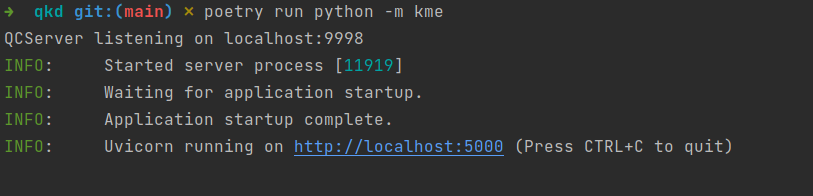
\includegraphics[width=0.9\textwidth]{Images/kme_start.png}
    \caption{A Key Management Entity started in a Linux terminal.}
    \label{fig:kme_start}
\end{figure}

\section{The web API interface}
\label{kme:api}

Thanks to FastAPI, one of the project's dependencies, the KME makes an API interface available as a web page by default. The KME displays the URL link to this interface in the terminal just after starting. The following figure shows an overview of the web page: it shows all the SAE's methods to interact with the KME. The web API interface can simulate the execution of an HTTP request to the KME.

\begin{figure}[H]
    \centering
    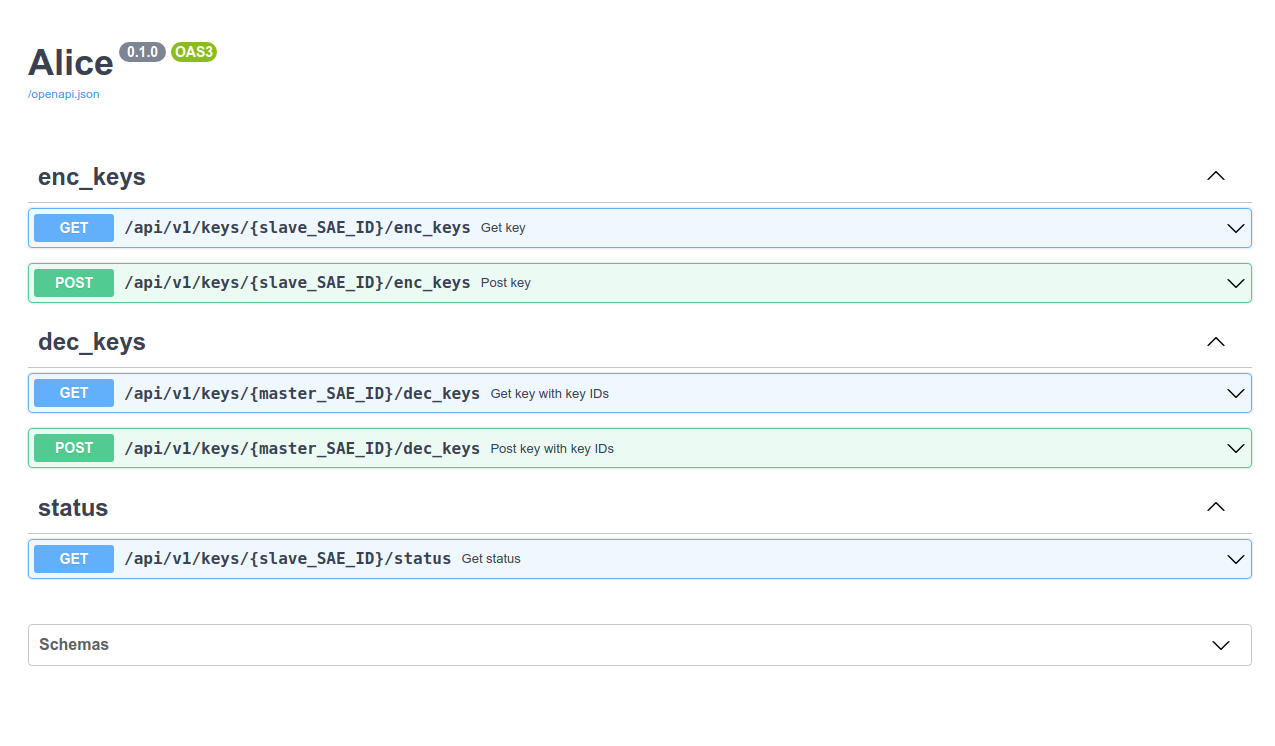
\includegraphics[width=1.0\textwidth]{Images/openapi.png}
    \caption{The web API interface made available by the KME thanks to FastAPI.}
    \label{fig:openapi}
\end{figure}

\begin{figure}[H]
    \centering
    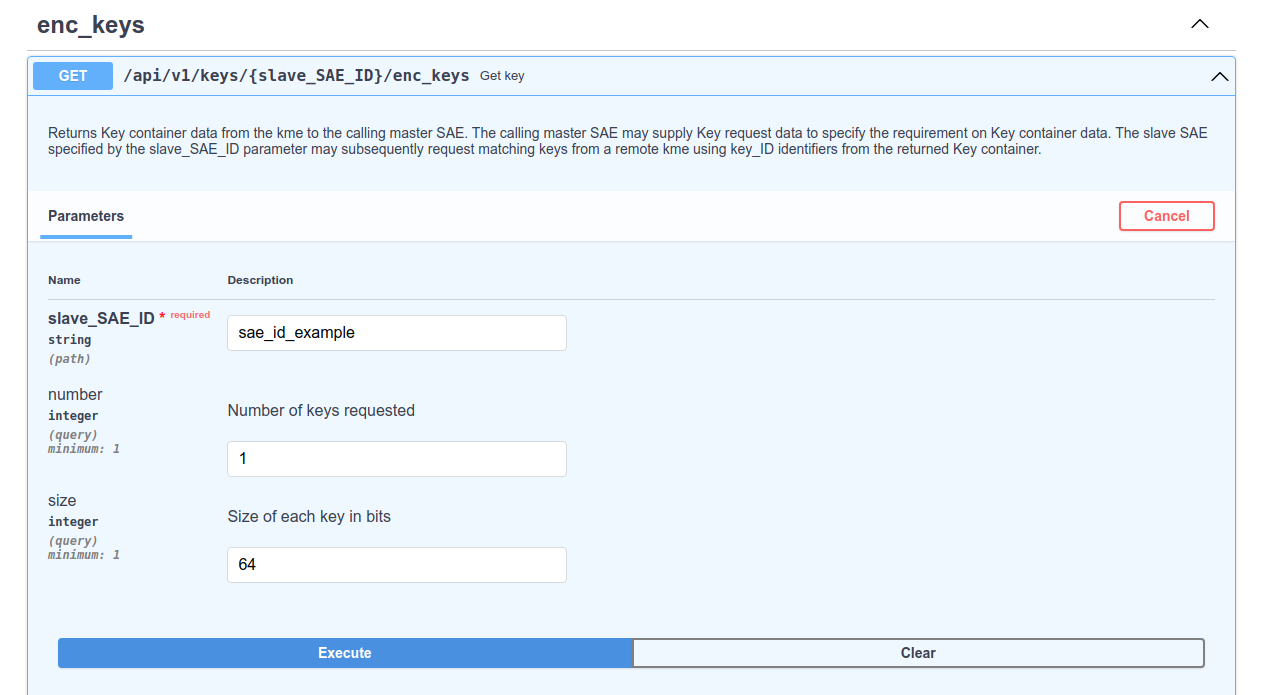
\includegraphics[width=1.0\textwidth]{Images/openapi_enc_keys.png}
    \caption{The simulation of a key generation request through the web API interface.}
    \label{fig:openapi_enc_keys}
\end{figure}

It is worth noting that FastAPI does not require explicit writing of these APIs: they are automatically created starting from the Python code written by the programmer. For example, here follows the signature of the Python function handling any HTTP GET request to the API \textit{/dec\_keys}:

\begin{minted}{python}
@router.get(path="/{master_SAE_ID}/dec_keys")
async def get_key_with_key_i_ds(
    master_SAE_ID: str,
    key_ID: UUID
) -> KeyContainer:
    ...
\end{minted}

FastAPI knows that the function is handling the API route \textit{/dec\_keys} thanks to the first line of code specifying the handled URL path. Then, FastAPI can retrieve the URL parameters required because they are the exact parameters of the Python function defined above. Moreover, FastAPI knows the JSON data format of the HTTP response body because it is of the same type specified as a return value for the Python function. For more information about how FastAPI can map Python functions to OpenAPI specifications, please refer to FastAPI documentation.

\section{Different modes of execution}
By default, the KME is started in "development mode": this is the environment used by the programmer while writing software. When the programmer wants to test the functioning of the project, it enters the so-called "testing mode". Then, the KME can be executed in "production mode" when the software is ready to be delivered. The choice of one environment changes some values of the configuration files. For example, the databases used in testing mode are not the same used in production mode. In Linux-based operating systems, it is possible to set the environment mode with the command:

\begin{minted}{bash}
export env=test
\end{minted}

Where the word "test" stands for "testing environment". Replace "test" with "dev" for explicitly activating the development environment; replace it with the word "prod" for activating the production environment. The same behavior can be achieved on the Windows command line with the command:

\begin{minted}{bash}
set env=test
\end{minted}

\section{The configuration file}
The project contains a configuration file that specifies important parameters relative to the KME behavior at runtime. Here follows a list of the main configuration parameters, whose overview may help to understand the way the different parts of the KME interact with each other:

\begin{itemize}
    \item KME\_ID: the ID of the KME. There is no standard way to specify the ID of a Key Management System. Therefore, we decided to call the two KMEs connected through the same quantum channel "Alice" and "Bob" in this project.
    \item HOST: the IP address \cite{ip} where the KME will run. By default, its value is "localhost", the network interface used to access network services running on the same host of the KME.
    \item PORT: the TCP port  \cite{tcp} where the KME will be listening to requests from SAEs.
    \item QC\_HOST: the IP address where the KME will be listening for new blocks coming from the quantum channel. By default, its value is also "localhost".
    \item QC\_PORT: the TCP port where the KME will be waiting for new blocks from the quantum channel.
    \item COMPANION\_URL: the URL where the cooperating KME is reachable. For example, suppose Alice is listening on "http://localhost:5000," and Bob is listening on "http://localhost:3000". In that case, Alice will have stored the listening URL of Bob, and vice versa.
    \item DEBUG: a Boolean flag whose value is True if debugging features enable is desired. When the KME is run in testing or development mode, this flag is set to True; it is set to False when in development mode.
    \item TESTING: a Boolean flag whose value depends on the running mode of the KME. In particular, it is True when the KME is run in testing mode, False otherwise. For more information about the testing mode, please see \ref{testing}.
\end{itemize}

\section{Quantum Channel Simulator}
\label{kme:qcs}

The implemented KME can communicate with Quantum Channels following the rules described in \ref{kme:qc}. However, working on the implementation of the KME, it was not always possible to communicate with the Quantum Channel in Politecnico di Milano. So, a piece of software simulating the behavior of a quantum channel was needed. Therefore, a Quantum Channel Simulator was implemented. This Quantum Channel Simulator does not provide the security strengths of a real Quantum Channel, and it is not intended for production purposes. However, it is convenient for testing and development environments. In order to start the Quantum Channel Simulator, the following command must be executed:

\begin{minted}{bash}
poetry run python -m qcs
\end{minted}

After starting the Quantum Channel Simulator, the KMEs connected will start receiving blocks. Therefore, they will be able to generate keys and perform all other tasks for which they were created.

As already mentioned, the material contained inside the blocks produced by the simulator is not the result of a Quantum Key Distribution Protocol. They are produced exploiting the function \textit{getrandbits()}, that is a function of the Python module called \textit{random}. Here follows the implementation of the function \textit{get\_random\_bits}, which is the core of the simulation of the generation of random bits:

\begin{minted}{python}
def get_random_bits() -> tuple[int, ...]:
    from random import getrandbits, randint

    # Generate a number of random bytes btw [lb, ub].
    lb, ub = 1000, 2000
    return tuple(getrandbits(8) for _ in range(randint(lb, ub)))
\end{minted}

The above Python code produces a pseudo-random number of pseudo-random bytes. The randomness depends on the internal implementation of the Python module \textit{random}, which is not based on QKD. So, once again, it is essential to notice that this simulator should not be exploited in an actual use case scenario.

Also, the number of bytes returned by the function is not deterministic. It is a value established by the function \textit{randint()}, that is also part of the Python module \textit{random}. This implementation choice aims at reproducing the behavior of a QKD protocol, which cannot determine the length of the block material \textit{a priori}, as discussed in \ref{kme:keys_vs_blocks}.

\section{Testing}
\label{testing}

When writing a software project, it is essential to write tests that are pieces of code intended to check that a given functionality is working as expected, despite the project's growth. Without a valid test suite, it is possible to modify part of the code introducing unexpected bugs.

Here, we exploited a Python test suite called \textit{pytest}. Thanks to \textit{pytest}, it is possible to execute all the tests written for the KME altogether with a single command:

\begin{minted}{bash}
poetry run pytest
\end{minted}

When the above command is executed, \textit{pytest} looks for all the files whose names start with the word "test". Then, inside such files, it looks for functions starting with the same prefix and executes them. This approach makes it easy to automate the testing phase. Each time the project is updated, it is possible to check the behavior of the KME executing the above command.

This KME implementation passes all the fifteen tests written for it. It is possible to read all the tests written for the KME inside the "tests" folder of the project.

\begin{figure}[H]
    \centering
    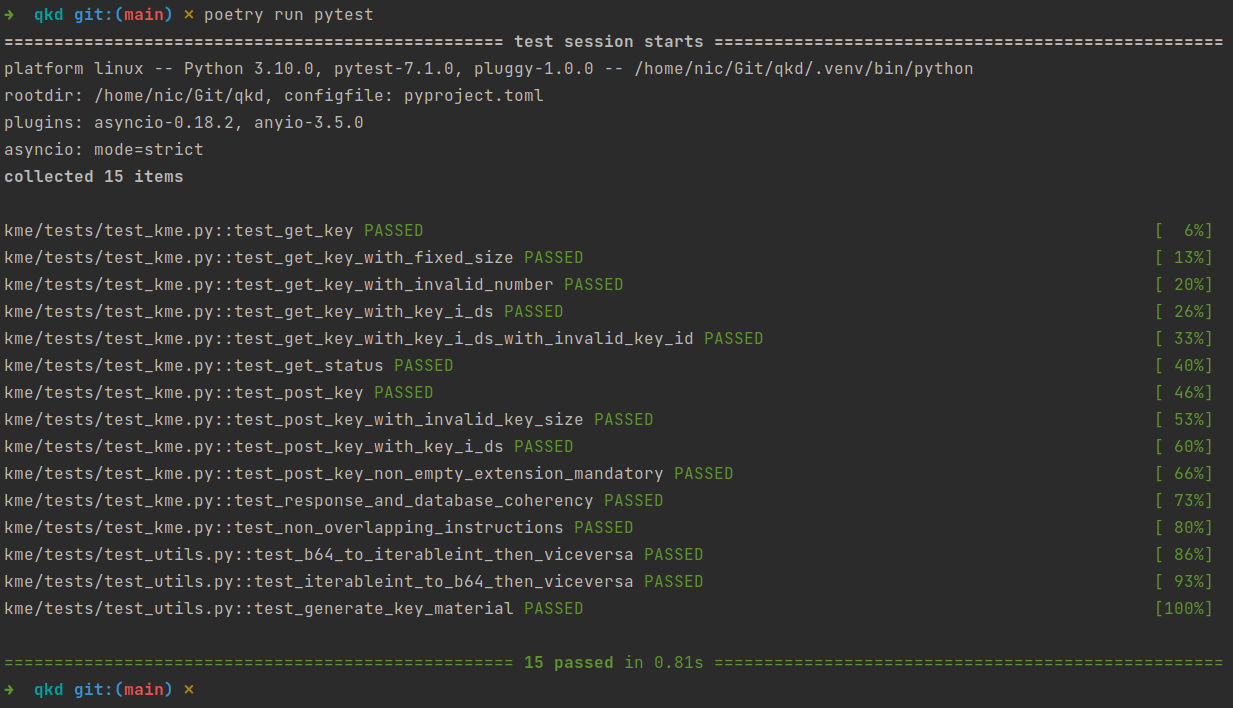
\includegraphics[width=1.0\textwidth]{Images/pytest.png}
    \caption{The result of the execution of the test suite with pytest.}
    \label{fig:pytest}
\end{figure}

Another critical aspect of testing is code coverage. The executed test suite should involve all the lines of code of the project. However, this is not sufficient to ensure that the project is free from bugs. In order to test the code coverage, this project exploits another Python package called "coverage". In order to run a test coverage, it is enough to execute the following command:

\begin{minted}{bash}
poetry run coverage report
\end{minted}

At the time of writing, the coverage of the project is near 94\%, which is considered a fair coverage value.

\begin{figure}[H]
    \centering
    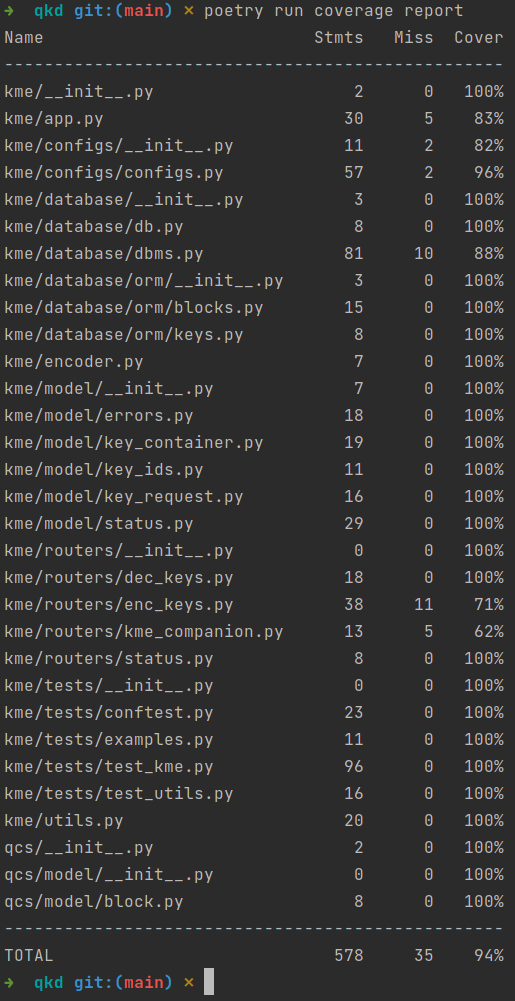
\includegraphics[width=0.6\textwidth]{Images/coverage.png}
    \caption{The result of the execution of the coverage test.}
    \label{fig:coverage}
\end{figure}

\section{Asynchronicity}
A notable feature of this implementation of a Key Management Entity is its ability to handle multiple Secure Application Entities requests concurrently. A great effort has been spent to make this KME implementation able to manage requests asynchronously. The concept of asynchronicity can be well explained through an example use case. 
Consider two Secure Application Entities, SAE A and SAE B, making requests to the same Key Management Entity. SAE A asks to create 50 new keys that are 2048 bits long. Then, SAE B asks for the key associated to the UUID 5835e93e-5250-4a85-b5d0-20ddf10e2f12. Notice that the request of SAE A requires an effort that is significantly greater than the one required for handling the request by SAE B. In a synchronous context, SAE B would receive the response to its "light" request only after SAE A has received its response. Instead, SAE B may receive its response before SAE A in this asynchronous context.
Moreover, suppose other Secure Application Entities send requests to the KME that are relatively easy to manage. In that case, the KME may send them a response while working on the answer to SAE A. The asynchronous management of the requests may significantly improve the performance of the KME.

The implementation of these features relies on Python's syntax, which allows defining a function with a signature that starts with the keyword \textit{async}. Lines of code that can be executed asynchronously inside an async function starts with the keyword \textit{await}. Indeed, while the Python interpreter is waiting for the result of an asynchronous request, it can devote time to handling other requests. For example, consider the following lines of code:

\begin{minted}{python}
async def generate(size: int) -> Key:
    key_id = uuid4()
    key_material, instructions = await generate_key_material(size)

    await orm.Key.objects.create(key_id, instructions)

    return Key(key_id, key_material)
\end{minted}

The one above is the function for creating one new key of fixed length. The second line of the function calls another function, \textit{generate\_key\_material}, devoted to the creation of key material, starting from blocks. This operation may be expensive in terms of time. So, while waiting for its termination, Python handles other requests. Finally, when the new key is generated, the third line of code is executed: it stores the instructions of the newly-generated key into the shared database. Also, this operation may be expensive, so it is "awaited". In the end, the new key is returned to the calling function.

One crucial aspect of asynchronicity is access to the databases. Indeed, making queries to a database is an expensive operation. This project uses a Python package called "orm", which allows making asynchronous queries to the database. Queries that only want to read the content of the database can be managed concurrently without worrying about the order they are made. Instead, two concurrent accesses to the local database for retrieving a block fragment are dangerous: they should not receive the same block fragment as a response. This behavior would lead to the exploitation of the same block material to build distinct keys, which is not the desired effect. Therefore, when one function requests a block fragment, that fragment is popped up from the database and is returned only to that function. When the function ends the exploitation of the block, if there are unexploited block material bits left, it re-inserts the updated block fragment inside the database.

The entire implementation of this KME is asynchronous: the management of requests to the API, the access to the databases, and the testing phase. This feature leads to the performance benefits previously described.